%
% main.tex -- Paper zum Thema <thema>
%
% (c) 2018 Nicolas Tobler, Hochschule Rapperswil
%

\chapter{Klima auf anderen Planeten\label{chapter:thema}}
\lhead{Klima auf anderen Planeten}
\begin{refsection}
\chapterauthor{Nicolas Tobler}

\section{Einleitung}

\rhead{Einleitung}
\begin{figure}
	% https://www.astrobio.net/news-exclusive/comparing-climates-from-earth-to-exoplanets/
	\centering
	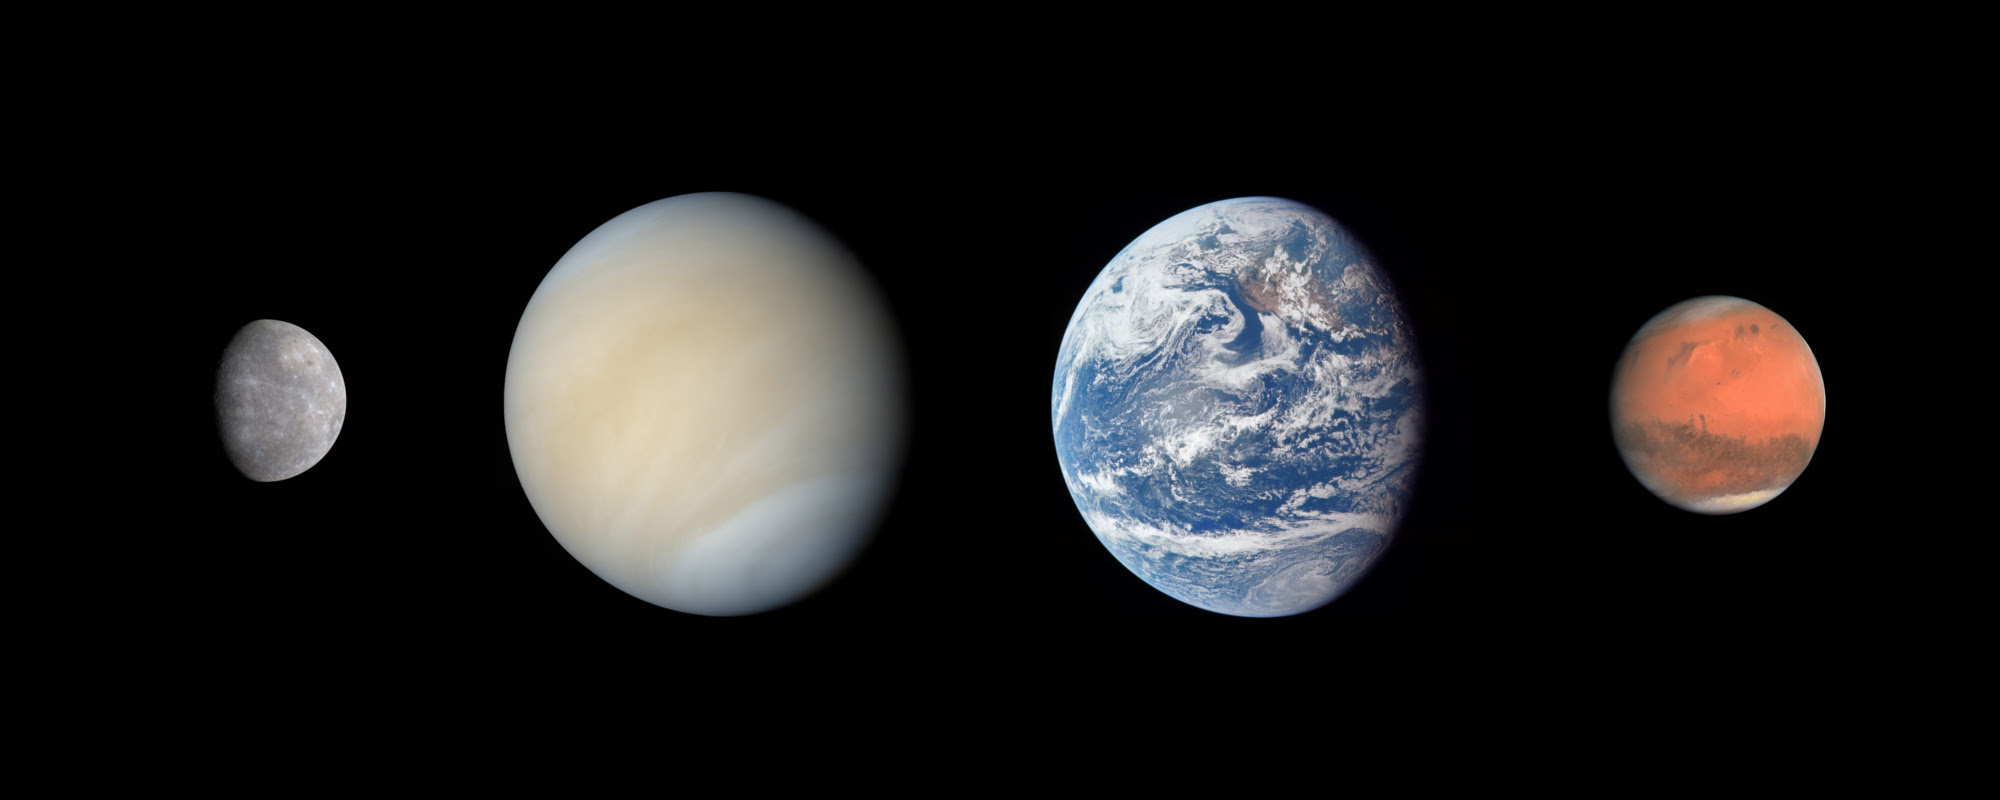
\includegraphics[width=0.7\linewidth, trim={0 2cm 0 2cm},clip]{planeten/Pictures/planets2.jpg}
	\caption{Merkur, Venus, Erde und Mars massstabsgerecht}
	% https://www.universetoday.com/13969/color-of-mercury/
	% https://medium.com/planet-stories/whats-false-about-true-color-2951ea5a4b5a
	% http://www.planetary.org/blogs/emily-lakdawalla/2009/2105.html
	% https://upload.wikimedia.org/wikipedia/commons/0/02/OSIRIS_Mars_true_color.jpg
\end{figure}

%Betrachtet man die vier der Sonne am nächst stehenden Planeten Merkur, Venus, Erde und Mars, gibt es einige Dinge festzustellen.
%Nur erde enthält leben
Die Erde ist aus heutiger Sicht der einzige Planet der Leben haltet. Trotz allen Einwirkungen über vier Milliarden Jahre sind wir in der glücklichen Lage auf der Erde ein mildes Klima vorzufinden, das das irdische Leben erhielt. 
Der Astrobiologe David Grinspoon meint dazu folgendes:
\begin{quote}
\textit{“It may be that conditions for life’s origin aren’t rare, but the hard part is the persistence of habitable conditions.”}
\begin{flushright}
--- David Grinspoon, Astrobiologe \cite{planeten:AstrobiologyMagazine} %% https://www.space.com/21234-alien-planets-earth-climate-future.html
\end{flushright}
\end{quote}
Es könnte also sein, dass auf den meisten Planeten im Sonnensystem einmal gute Voraussetzungen für leben bestanden. Aber nur die Erde konnte mit einem anhaltenden, lebensfreundlichen Klima das Leben aufrecht erhalten.

Die für Leben wahrscheinlich wichtigsten Konditionen sind flüssiges Wasser und dadurch auch milde Temperaturen. Flüssiges Wasser nur noch auf der Erde in grossen Mengen auffindbar.
%Andere Planeten andere entwicklung
Alle anderen Planeten konnten offenbar kein freundliches Klima bewahren. Tabelle \ref{planeten_comparison} zeigt ein Vergleich der vier sonnennächsten Planeten.
\begin{center}
\begin{table}
	\center
	\begin{tabular}{l|c c c c}
							& Merkur			& Venus				& Erde		& Mars                  \\
  \hline
  Oberflächen Temperatur	& 452 K				& 733 K				& 287 K		& 226 K                 \\
  Wasser auf Oberfläche		& -					& -					& Ozeane	& Polares Eis			\\
  Wasser in Athmosphäre		& -					& $0.002\%$ 		& $0.4\%$	& Spuren				\\
  Wolken					& -					& $\approx100\%$	& $67\%$  	& $<5\%$                \\
  Atmosphäre				& $10^{-15}$ bar	& $92$ bar			& $1$ bar	& $6 \cdot 10^{-3}$ bar 
	%\hline
\end{tabular}
% (http://www.climate4you.com/ClimateAndClouds.htm) not used yet
\caption{Planeten im Vergleich \cite{planeten:temperatures} \cite{planeten:cloudcover}}
\label{planeten_comparison}
\end{table}
\end{center}
Die planetaren Wassermassen gefroren unter der Oberfläche oder entwichen es ins All. Letzterer Fall ist besonders schlimm, da der Vorgang irreversibel ist. Der Planet verliert somit seine lebensfreundliche Lage für immer.

Doch wie kommen diese extremen Konditionen zu Stande? Man könnte meinen, dass primär die Distanz zur Sonne für die Temperatur ausschlaggebend ist. Jedoch diese über die Planeten mit der Entfernung zur Sonne nicht stetig ab.
%Wegen anderen parametern?
Das Klima muss somit auch von anderen Parametern abhängig sein, wie zum Beispiel Durchmesser, Rotation, Vulkanismus, Magnetfeld und viele andere.
%Aufgrund orbitalen parameter?
In diesem Kapitel gehe ich der Frage nach, ob Venus und Mars alleine aufgrund ihrer orbitalen Eigenschaften nicht fähig waren, ein lebensfreundliches Klima zu generieren. Die Nullhypothese lautet somit, dass die genannten Planeten durch ihre Umlaufbahn oder Grösse \textit{nicht} benachteiligt sind, lebensfreundliche Klimabedingungen zu halten.

%Könnte es der Erde in Zukunft auch gleichermassen ergehen?
%Was führt zu wasserlosen Atmosphäre?

\section{Ziel}
Es soll ein Modell erstellt werden, welches das Klima von Planeten mit deren orbitalen Eigenschaften verknüpft.
Betrachtet wird ein früher Zeitpunkt der Geschichte des Sonnensystems, als die Planeten ähnliche oder annähernd gleiche materielle und atmosphärische Bedingungen aufwiesen.
Mit der Annahme, dass grosse Mengen an Wasser auf allen Planeten vorhanden war, besteht auf allen Planeten die gleichen Voraussetzungen für mögliches Leben.
In das gleiche Modell werden für jeden Planeten deren unterschiedlichen orbitalen Parameter eingesetzt. Man kann sich das vorstellen, als nehme man zum Beispiel die Erde, skaliert sie auf Mars-Grösse und setzt sie in den Mars-Orbit. 
Durch eine Simulation des Modells im Zeitbereich sollte dann eine Aussage über den Werdegang der Planeten gemacht werden.

\section{Modell}
\rhead{Modell}


	%Das Modell muss einige Sachen erfüllen, um eine Aussage machen zu können.
	
	%Das Modell wird so allgemein gehalten um für alle Planeten 

	%1. Für alle Planeten geltendes Modell erstellen
	
	%2. Modell soll 
	
	
	Das hier erarbeitete Modell muss für alle untersuchen Planeten gelten. Deshalb konzentriert es sich nur auf die Strahlungsbilanz und den Wasserkreislauf. Es wird davon ausgegangen, dass das Wasser signifikant für das Klima ist, da atmosphärischer Wasserdampf auf der Erde den grössten Anteil zum Treibhauseffekt beisteuert. Ausserdem befinden sich alle betrachteten Planeten in der habitablen Zone, auch Bekannt als Goldilocks Zone. Diese beschreibt den Abstandsbereich um die Sonne, in dem flüssiges Wasser dauerhaft auftreten kann.
	Andere klimabestimmenden atmosphärischen Gase wie $\text{CO}_\text{2}$ werden nicht simuliert, um das Modell im gegebenen Rahmen umzusetzen.
	Das Modell sollte erdähnliche Bedingungen bewusst anstreben, um zu sehen ob diese auf den Planeten Mars und Venus auch bestehen können.
	
Auf Grund der zum Teil starken Vereinfachungen müssen einzelne Parameter abgeschätzt werden. Durch diese freien Parametern kann das System getrimmt werden um überhaupt plausible Lösungen zu erreichen. Diese Parameter sind mit $\xi$'s gekennzeichnet.

\begin{figure}
	\centering
	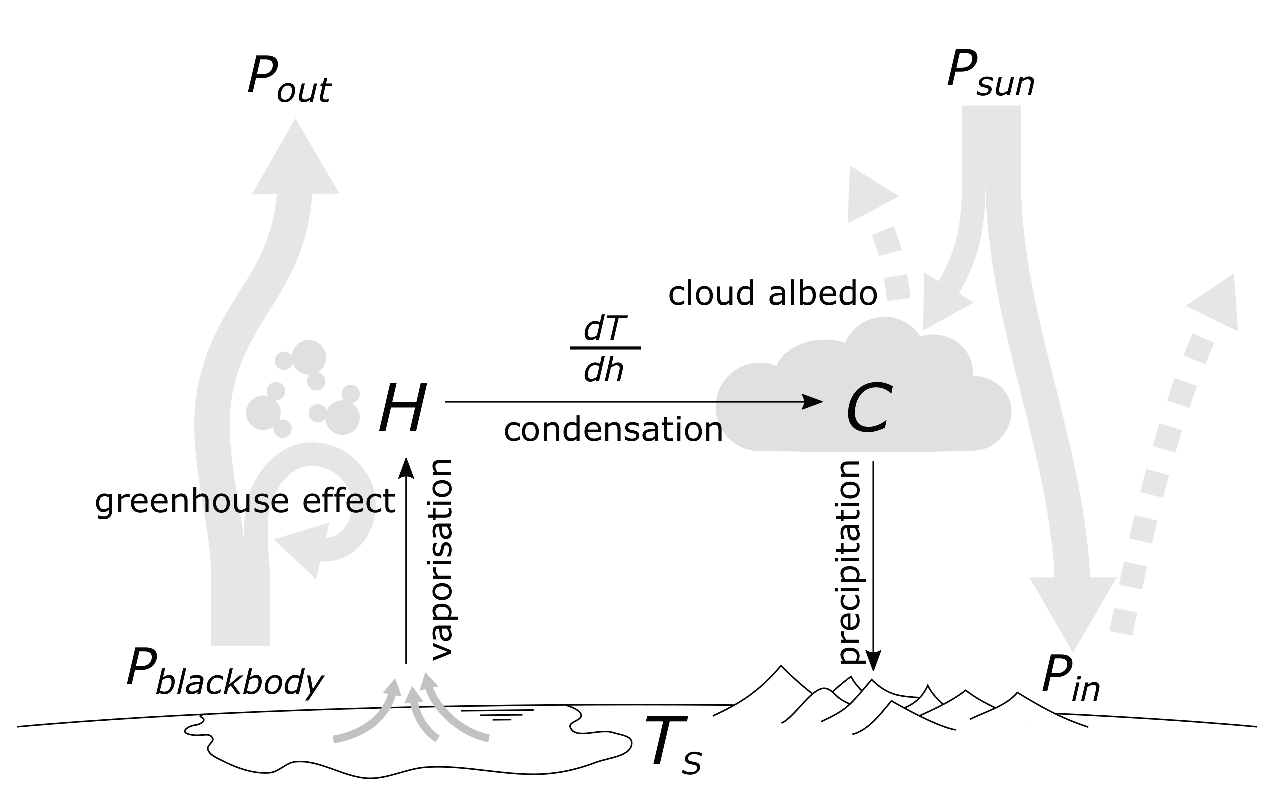
\includegraphics[width=0.8\textwidth]{planeten/Pictures/Model.eps}
	\caption{Modell-Übersicht}
	\label{planeten:model}
\end{figure}
Abbildung \ref{planeten:model} zeigt eine Übersicht des Modells.
Das Modell hat die Form eines Differentialgleichungssystems, wobei folgende drei Parameter modelliert werden:
\begin{itemize}
\item [\textbf{Surface temperature $T_s$}]	Mittlere Oberflächentemperatur des Planeten
\item [\textbf{Clouds $C$}]		Wolkenabdeckung zwischen 0 und 1
\item [\textbf{Humidity $H$}]		Atmosphärischer Wasserdampf zwischen 0 und 1
\end{itemize}
Die Parameter $C$ und $H$ können näherungsweise als prozentuale Wolkenabdeckung beziehungsweise relative Luftfeuchtigkeit  interpretiert werden.
Das Modell wird für die Planeten Merkur, Venus, Erde und Mars simuliert, wobei deren Mittlere Distanz $a_\text{planet}$ zur Sonne und Radius $R_\text{planet}$ eingesetzt werden.

\subsection{Strahlungsbilanz}
Die Strahlungsbilanz wird im Kapitel \ref{skript:subsection:strahlungsbilanz} ausführlich beschrieben. Das hier verwendeten Modell baut direkt darauf auf.

Damit die Durchschnittstemperatur eines Planeten stabil ist, muss die Leistungsbilanz Null sein:
\begin{equation}
\dot{T}_S \propto P_{\text{in}} - P_{\text{out}}\text{ .}
\end{equation}
Die Planeten sind jedoch nicht gleich gross. Damit die Auswirkung eines Strahlungsungleichgewicht für alle Planeten gleich ist, muss die Leistung auf eine Flächeneinheit normalisiert werden. Somit hat eine Stück Fläche mit der Atmosphäre darüber auf jedem Planeten die gleiche Wärmekapazität. Mit normalisierung ist
\begin{equation}
\dot{T}_S = \xi_1 \frac{P_{\text{in}} - P_{\text{out}}}{A} = \xi_1 \frac{P_{\text{in}} - P_{\text{out}}}{4 \pi R_{\text{planet}}^2}\text{ .}
\end{equation}

Wie in Kapitel \ref{skript:grundlagen:strahlung} beschrieben, wird die Solarkonstante
\begin{equation}
P_{\text{solar}} = \sigma T_{\astrosun}^4 \left( \frac{R_{\astrosun}}{a_{\text{planet}}} \right) ^2
\end{equation}
aus der Entfernung $a_{\text{planet}}$ des Planeten zur Sonne berechnet. Multipliziert mit der zur Sonne zeigenden Querschnitsfläche $\pi R_{\text{planet}}^2$ ergibt sich die total auftreffende Leistung. Diese wird teils von der Albedo $\alpha$ reflektiert. Zurück bleibt die vom Planeten absorbierte Leistung \begin{equation}
P_{\text{in}} = P_{\text{solar}}  \pi R_{\text{planet}}^2 (1-\alpha) = \sigma T_{\astrosun}^4 \left( \frac{R_{\astrosun}}{a_{\text{planet}}} \right) ^2 \pi R_{\text{planet}}^2 (1-\alpha)\text{ .}
\end{equation}
Andere Energiequellen neben der Sonne wie Geothermie oder Gezeitenkräfte werden vernachlässigt.

Aus dem Radius und Oberflächentemperatur $T_{S}$ eines Planeten wird deren Schwarzkörper-Strahlung \begin{equation}
P_{\text{blackbody}} = 4 \pi R_{\text{planet}}^2 \sigma T_{S}^4
\end{equation}
berechnet. Diese Leistung bleibt jedoch teilweise durch den Treibhauseffekt $\beta$ in der Atmosphäre gefangen. Der Anteil der durchdringenden Leistung ist
\begin{equation}
P_{\text{out}} = P_{\text{blackbody}} (1 - \beta) = 4 \pi R_{\text{planet}}^2 \sigma T_{S}^4 (1 - \beta)\text{ .}
\end{equation}

\subsection{Albedo}
Die Albedo $\alpha$ wird als Funktion der Wolkenabdeckung $C$ modelliert. Es wird ein linearer Zusammenhang erwartet. Sie ist begrenzt durch die zwei Werte
\begin{equation}
\alpha_{\text{min}} = 0.15 \text{ und } \alpha_{\text{max}} = 0.48 \text{ .}
\end{equation}
Die minimale Albedo $\alpha_{\text{min}}$ tritt bei 0\% Wolkenabdeckung auf und hat den Wert der Albedo des Mondes, der kleinsten in unserem Sonnensystem. Die maximale Albedo $\alpha_{\text{max}}$ tritt bei 100\% Wolkenabdeckung auf und wird so gesetze, dass bei der Wolkenabdeckung der Erde die Erdalbedo resultiert. Somit ist
\begin{equation}
\alpha = \alpha_{\text{min}} + C(\alpha_{\text{max}} - \alpha_{\text{min}}) \text{ .}
\end{equation}

\subsection{Treibhauseffekt}
Wasserdampf ist ein sehr effektives Treibhausgas. Es wird angenommen, dass der atmosphärische Wasserdampf der Erde für 60\% des Treibhauseffekts sorgt. \cite{planeten:treibhauseffekt}  
Im verwendeten Modell wirkt sich deren Konzentrazion $H$ linear auf den Teibhauseffekt 
\begin{equation}
\beta  = \beta_{\text{max}} \cdot H
\end{equation}
aus. Die Wirkung wird mit $\beta_{\text{max}}$ beschränkt und kann vor der Simulation justiert werden.

Die Strahlungsbilanz kann somit mit
\begin{equation}
\dot{T}_S = \xi_1 \frac{\sigma T_{\astrosun}^4 R_{\astrosun}^2}{4 \pi R_{\text{planet}}^2 a_{\text{planet}}^2} (\alpha_{\text{min}} + C(\alpha_{\text{max}} - \alpha_{\text{min}})) - \xi_1 \sigma T_{S}^4  (1 - \beta_{\text{max}} \cdot H)
\end{equation}
zusammengefasst werden.

\subsection{Wasserkreislauf}
Das Modell beinhaltet einen stark vereinfachten Wasserkreislauf.
Dieser verknüpft die Parameter Clouds $C$ und Humidity $H$.
Dazu kommt das auf der Planetenoberfläche vorhandene flüssige Wasser, welches als Quelle und Senke dient und zugleich unerschöpflich ist. Das Modell beachtet nicht, dass der atmosphärische Wasserdampf ins All entweichen kann und dadurch die Ozeane austrocknen können. Zwischen den Parametern gibt es die drei Flüsse $h_{\text{Wasserdampfbildung}}$, $h_{\text{Wolkenbildung}}$ und $h_{\text{Wolkenabbau}}$. Diese bilden das folgende Gleichungssystem:
\begin{equation}
\begin{matrix}
\dot{H}   = & h_{\text{Wasserdampfbildung}} & - h_{\text{Wolkenbildung}}   &                      \\
\dot{C}   = &                     		    &   h_{\text{Wolkenbildung}}   & - h_{\text{Wolkenabbau}}
\end{matrix} \text{ .}
\end{equation}

%\subsubsection{Wasserdampfbildung}
Wasserdampf bildet sich durch Verdunsten von der Ozeane. Der Durchsatz wird linear zur Oberflächentemperatur $T_S$ angenommen und ist dadurch
\begin{equation}
h_{\text{Wasserdampfbildung}} = \xi_2 T_S \text{ .}
\end{equation}


%\subsubsection{Wolkenbildung}
Wolken entstehen, wenn feuchte Luft beim aufsteigen sich abkühlt und kondensiert. Näherungswiese entstehen mehr Wolken je grösser die Luftfeuchtigkeit $H$ ist und je schneller die Temperatur mit der Höhe abnimmt.
Dabei nimmt die Wolkenbildung mit grösserer Luftfeuchtigkeit $H$ und grösserem Temperaturgradienten $\frac{dT}{dh}$ zu. Durch Multiplizieren mit einem wählbaren Parameter $\xi_3$ kann die Wirkung des Prozesses justiert werden. Die Wolkenbildung ist somit
%Wolken bilden sich durch kondensieren des Wasserdampfs. Dieser Vorgang
%feuchte Luft abgekühlt wird
%bei grossem Temperaturgradienten
\begin{equation}
h_{\text{Wolkenbildung}} = \xi_3 H \frac{dT}{dh} \text{ .}
\end{equation}

%TODO Cite website
Der Temperaturgradient existiert sowohl in vertikaler, sowie in horizontaler Ausrichtung. Einen grossen horizontalen Gradienten findet man zum Beispiel bei einer Wetterfront vor, wenn unterschiedlich warme Luftmassen aufeinander treffen. Im Modell wird nur der vertikale berücksichtigt, welcher auf der Erde ca. $1$ Kelvin pro $100$ Meter entspricht. Dieser ist bei ungesättigter Luft annähernd konstant. Sobald Wasserdampf kondensiert wird der Prozess feuchtadiabatisch und der Gradient wird kleiner. Linear approximiert ergibt sich dadurch
\begin{equation}
h_{\text{Wolkenbildung}} = \xi_3 H \frac{dT}{dh} = \xi_3 H \frac{1}{C} \text{ .}
\end{equation}

%\subsubsection{Wolkenabbau}
Wolken regnen, wenn sich die mikroskopischen Wassertropfen oder Eiskristalle verbinden und nicht mehr getragen werden können. Im hier verwendeten Modell wird angenommen, dass sich Regenbildung somit proportional zur Wolkenabdeckung $C$ verhält. Somit ist
\begin{equation}
h_{\text{Wolkenabbau}} = \xi_4 C \text{ .}
\end{equation}


%\subsection{Zusammengefasst}
%Der ganze Wasserkreislauf lässt sich somit durch folgendes Gleichungssystem zusammenfassen.
%
%\begin{equation}
%	\begin{matrix}			
%		\dot{H} = & \xi_2 P_{\text{in}}(C) & - \xi_3 H \Delta T & \\
%		\dot{C} = &                        &   \xi_3 H \Delta T & - \xi_4 C
%	\end{matrix}	
%\end{equation}


%\subsection{Entweichen von atmosphärischen Gasen}
%
%Ob ein Planet oder Mond eine Atmosphäre besitzt ist von wenigen parametern abhängig. Planeten behalten ihr Atmosphäre, wenn die Gravitation ausreichend stark ist, um die Moleküle gegen ihre thermische Geschwindigkeit zurückzuhalten.
%Die Moleküle in der Atmosphäre, für die
%
%% https://www.tcd.ie/Physics/people/Peter.Gallagher/lectures/PY4A03/pdfs/PY4A03_lecture12n13_amospheres.ppt.pdf
%
%\begin{equation}
%v_{escape} > v_{therm}
%\end{equation}
%
%zutrifft, werden nach und nach in den Weltraum abgestossen.
%Die Fluchtgeschwindigkeit eines Planeten $v_{escape}$ wird durch deren Masse $M$ und Radius $R$ berechnet: 
%
%\begin{equation}
%v_{escape} = \sqrt{\frac{2GM}{R}}
%\end{equation}
%
%wobei $G$ die Gravitationskonstante ist. Die Fluchtgeschwindigkeit ist somit bei grossen und schweeren Gestirnen grösser.
%
%Die thermische Geschwindigkeit eines Moleküls ist Maxwell-Bolzmann-verteilt. Deshalb gilt der berechnete Wert in diesem Zusammenhang nur approximativ. Die höchst wahrscheinliche Geschwindigkeit ist: 
%
%\begin{equation}
%v_{therm} = \sqrt{\frac{3kT}{m}}
%\end{equation}
%
%Dabei ist $k$ die Bolzmann-Konstante und $m$ die Mol-Masse des Moleküls. Die kritische Temperatur $T_{escape}$, bei welcher Gase abgestossen werden ist somit:
%
%\begin{equation}
%T_{escape} = \frac{2GMm}{3kR}
%\end{equation}

\subsection{Gleichungssystem}

Durch Zusammenfassen von Strahlungsbilanz und Wasserkreislauf erhält man folgendes Gleichungssystem:
\begin{equation}
\begin{matrix}
\dot{T}_S = & \xi_1 \frac{\sigma T_{\astrosun}^4 R_{\astrosun}^2}{4 \pi R_{\text{planet}}^2 a_{\text{planet}}^2} (\alpha_{\text{min}} + C(\alpha_{\text{max}} - \alpha_{\text{min}})) && - \xi_1 \sigma T_{S}^4  (1 - \beta_{\text{max}} \cdot H)\\
\dot{H}   = & \xi_2 T_S              & - \xi_3 H \frac{1}{C}          & \\
\dot{C}   = &                        &   \xi_3 H \frac{1}{C}          & - \xi_4 C
\end{matrix} \text{ .}
\end{equation}
Um zu verhindern, dass eine Luftfeuchtigkeit oder Wolkenabdeckung von über 100\% auftritt, werden zu gewissen linearen Termen noch den gleichen Term mit grosser Potenz dazu addiert. Eine Funktion
\begin{equation}
f(x) = x \hspace{0.5cm}\text{wird zu}\hspace{0.5cm} f'(x) = x + x^n \text{ ,}
\end{equation}
wobei $n$ ungerade ist und somit auch $f'(x)$ ungerade bleibt. Der Effekt von $f'(x)$ wird für $x$ gegen $1$ exponentiell grösser und verstärkt den Term. Abbildung \ref{planeten:limit_graph} zeigt das Verhalten beider Funktionen.
\begin{figure}[!h]
	\center
	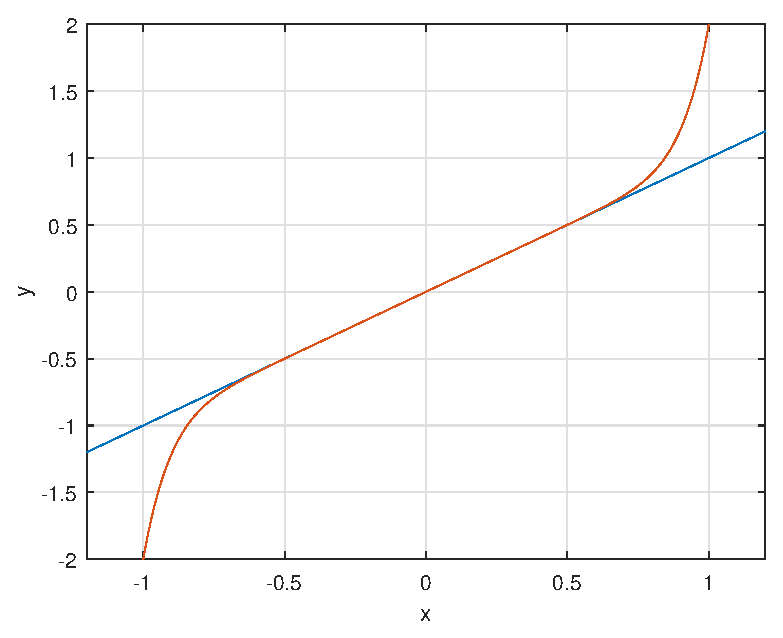
\includegraphics[height=0.45\textheight]{planeten/Matlab/figures/limiter.eps}
	\caption{Limitierung von Termen mit $f(x) = x$ in blau und $f'(x) = x + x^7$ in rot.}
	\label{planeten:limit_graph}
\end{figure}
Diese Art von Limitierung wird bei der Wolkenbildung, sowohl beim Wolkenabbau eingesetzt. Das fertige, angepasste Modell lautet somit:
\begin{equation}
\begin{matrix}
\dot{T}_S = & \xi_1 \frac{\sigma T_{\astrosun}^4 R_{\astrosun}^2}{4 \pi R_{\text{planet}}^2 a_{\text{planet}}^2} (\alpha_{\text{min}} + C(\alpha_{\text{max}} - \alpha_{\text{min}})) && - \xi_1 \sigma T_{S}^4  (1 - \beta_{\text{max}} \cdot H)\\
\dot{H}   = & \xi_2 P_{\text{in}}(C) & - \xi_3 (H + H^9) \frac{1}{C}   &                   \\
\dot{C}   = &                        &   \xi_3 (H + H^9) \frac{1}{C}   & - \xi_4 (C + C^5)
\end{matrix} \text{ .}
\end{equation}

\section{Simulation}
\rhead{Simulation}

Das Modell wurde in MATLAB mittels Transientenanalyse simuliert. Dazu kam ein ODE45 Solver zum Einsatz. Die Anfangswerte wurden so gesetzt, dass sie Erdbedingungen unterstützen.
\begin{equation}
\begin{matrix}
T_0 = & 287 \\
H_0 = & 0.44 \\
C_0 = & 0.67
\end{matrix}
\end{equation}sind Jahresmittelwerte von Oberflächentemperatur, Relativer Luftfeuchtigkeit, und Wolkenabdeckung.
Die in Tabelle \ref{planeten:xiValues} ersichtlichen freien Parameter $\xi_1$ bis $\xi_4$ sowie $\beta_{\text{max}}$ wurden empirisch gesetzt um für die Erde stabile Resultate zu erhalten.
\begin{center}
\begin{table}[!h]
	\center
	\begin{tabular}{c|c|l}
        & Wert                  & Beschreibung \\
  \hline
$\xi_1$ & $1$					& Wirkung der Leistungsdifferenz auf die Oberflächentemperatur\\
$\xi_2$ & $1.7 \cdot 10^{-2}$	& Koeffizient Wasserdampfbildung\\
$\xi_3$ & $2.8 \cdot 10^{0}$	& Koeffizient Wolkenbildung \\
$\xi_4$ & $5.1 \cdot 10^{0}$	& Koeffizient Wolkenabbau \\
$\beta_{\text{max}}$ & $0.5$	& Maximaler Anteil der durch den Treibhauseffekt zurückgehaltenen Leistung
	\end{tabular}
	\caption{Für die Simulation gesetzte freien Parameter}
	\label{planeten:xiValues}
\end{table}
\end{center}
In Tabelle \ref{planeten:planetValues} sind die für die Planeten eingesetzten Parametern $a_{\text{planet}}$ und $R_{\text{planet}}$ ersichtlich. Da der Orbit eines Planeten elliptisch sein kann, muss für $a_{\text{planet}}$ die Distanz zur Sonne über die Umlaufzeit gemittelt werden. Dieser Mittelwert kann aus den elliptischen Halbachsenparametern $a$ und $b$ berechnet werden \cite{planeten:umlaufbahn}:
\begin{equation}
a_{\text{planet}} = a \left(1+{\frac {e^{2}}{2}}\right) = \frac{3}{2}a - \frac{b^2}{2a} \text{ .}
\end{equation}
Dabei ist $e$ die Exzentrizität der Umlaufbahn.
Das System wurde bis zum stationären Zustand simuliert. Aus der Zeitachse können keine quantitative Schlüsse gezogen werden.
\begin{center}
\begin{table}[!h]
	\center
	\begin{tabular}{l|c c c c}
                        & Merkur                    & Venus                    & Erde                    & Mars     \\
  \hline
  $a_{\text{planet}}$   & $5.913 \cdot 10^{10}$ m   & $1.082 \cdot 10^{11}$ m  & $1.496 \cdot 10^{11}$ m & $2.289 \cdot 10^{11}$ m \\
  $R_{\text{planet}}$   & $2.439 \cdot 10^{6}$ m   & $6.0519 \cdot 10^{6}$ m  & $6.371 \cdot 10^{6}$ m  & $3.3895 \cdot 10^{6}$ m 
\end{tabular}
\caption{Für die Planeten eingesetzte Werte \cite{planeten:radius} \cite{planeten:semiMinorAxis}}
\label{planeten:planetValues}
\end{table}
\end{center}

\subsection{Ergebnisse}

	Abbildungen \ref{planeten:figSurfaceTemperature} bis \ref{planeten:figAlbedo} zeigen die Simulationsergebnisse in durchgezogenen Linien. Die Strich-Punkt-Linie der entsprechenden Farben zeigt den heutigen Wert der Grössen.
		
	Das simulierte Klima auf der Erde hat nur geringe Abweichungen zu den real gemessenen Werten. Das Modell wurde auch explizit für das Erdklima ausgelegt.
	
	Die Temperatur auf dem Mars ist ähnlich kalt wie heute beobachtbar. Obwohl eine aktive Troposphäre simuliert wird, kann die durchschnittliche Temperatur nicht über den Gefrierpunkt von Wasser steigen. Vermutlich kompensiert das durch die Wolken höhere Albedo den Treibhauseffekt. Das entstehende Eis würde das Albedo noch stärker erhöhen, was für noch tiefere Temperaturen sorgt. In äquatorialen Gegenden könnte flüssiges Wasser durchaus bestehen.
	
	Die Venus ist mit zirka 100$^\circ$C viel kälter als heute beobachtet, aber immer noch viel zu heiss um Flüssiges Wasser auf längere Zeit zu halten. In polaren Regionen sind die Temperaturen vermutlich milder und lebensfreundlicher.
	
	Merkur ist dank dem Treibhauseffekt einiges heisser wie heute beobachtbar. Die vorhandene Atmosphäre mit hohem Wasserdampfanteil erhöht die Temperatur enorm. Da Merkur allerdings verhältnismässig leicht ist und an starkem Sonnenwind ausgesetzt ist, wird diese Athmosphäre nicht lange bestehen.

		\begin{figure}
			\center
			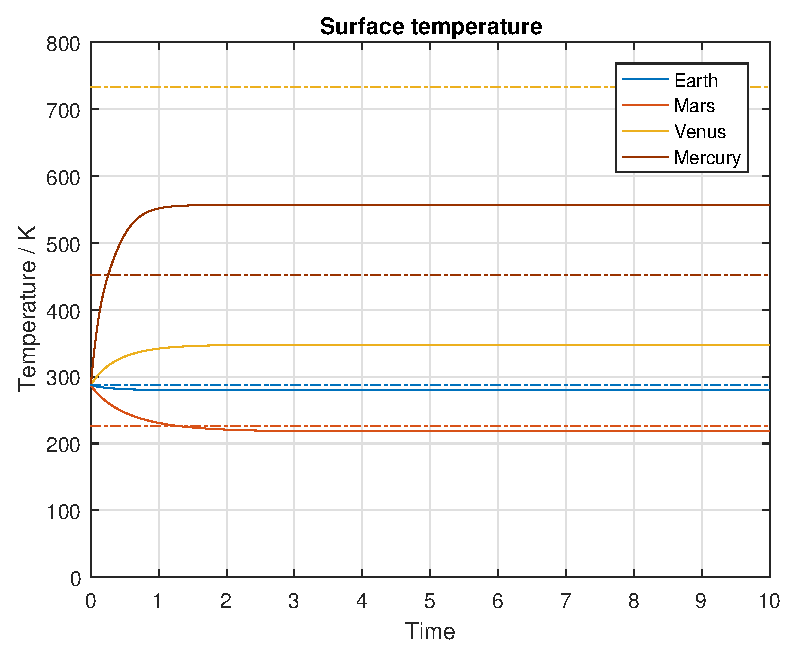
\includegraphics[height=0.45\textheight]{planeten/Matlab/figures/surfaceTemperature.eps}
			\caption{Globale Durchschnittstemperatur}
			\label{planeten:figSurfaceTemperature}
		\end{figure}
		
		\begin{figure}
			\center
			\includegraphics[height=0.45\textheight]{planeten/Matlab/figures/humidity.eps}
			\caption{Relative Luftfeuchtigkeit}
			\label{planeten:figHumidity}
		\end{figure}
		
		\begin{figure}
			\center
			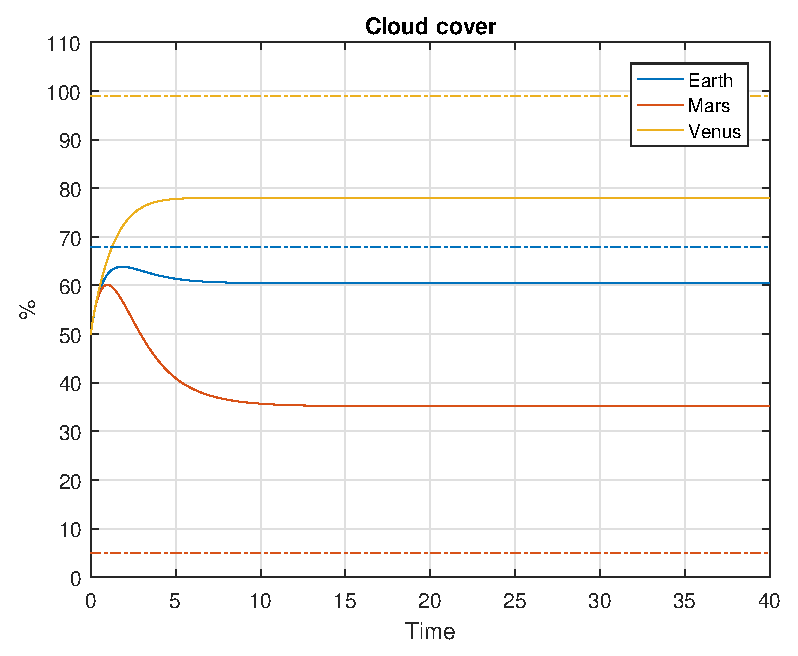
\includegraphics[height=0.45\textheight]{planeten/Matlab/figures/cloudCover.eps}
			\caption{Prozentuale Wolkenabdeckung}
			\label{planeten:figCloudCover}
		\end{figure}
		
		\begin{figure}
			\center
			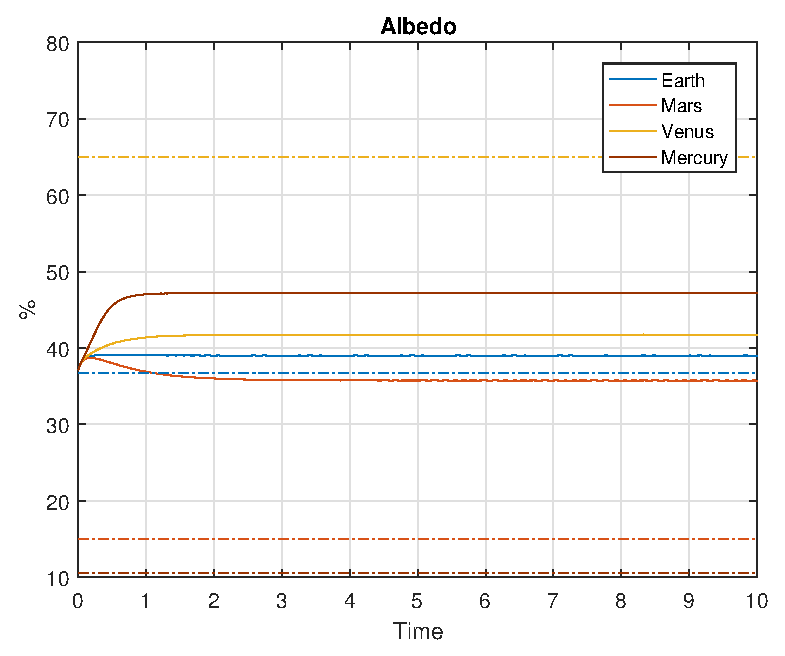
\includegraphics[height=0.45\textheight]{planeten/Matlab/figures/albedo.eps}
			\caption{Albedo}
			\label{planeten:figAlbedo}
		\end{figure}

\section{Schlussfolgerung}
\rhead{Schlussfolgerung}

Die Simulationsergebnisse tendieren zu den heute beobachtbaren Klimaverhältnissen. Die extremen Klimas von Mars und Venus sind somit vermutlich durch ihre Grösse und Umlaufbahn prädestiniert. Die Nullhypothese kann somit falsifiziert werden. Es können jedoch nur qualitative Schlüsse gezogen werden, da durch Verändern der freien Parameter ein ganz anderes Bild entsteht. Somit sind die Ergebnisse nur mit Vorsicht zu geniessen.

Abweichungen sind durch diverse Fehlerquellen gerechtfertigt. Zum einen wurden diverse chemische und physikalische Vorgänge bei extremen Temperaturen und Sonneneinstrahlung nicht beachtet.
Neben Wasser wurden Treibhausgase wie CO$_2$ vernachlässigt. Sie machen heute den grössten Anteil der Venus- und Marsatmosphäre aus.

\subsection{Verbesserungsmöglichkeiten}

Dieses Modell bietet diverse Ausbaumöglichkeiten. Um zum Beispiel mehr Genauigkeit in den Extremen Bereichen zu erreichen, müssten mehr atmosphärische Gase einbezogen werden.
Diese Gase besitzen wiederum unterschiedliche Gefrierpunkte, was die Modellierung der Vereisung zulässt.
		
Im simulierten Modell wurden lediglich der Durchmesser und die Distanz zur Sonne der Planeten einbezogen. Um die Aussagekraft zu verbessern könnten weitere klimabestimmende Parameter implementiert werden, die sich von Planet zu Planet unterscheiden. Mögliche Eigenschaften wären Vulkanismus und die Rotationsgeschwindigkeit. Die Rotation erlaubt das Modellieren von Tag- und Nachtseitentemperatur, welche sich stark auf das Klima auswirken.

\printbibliography[heading=subbibliography]
\end{refsection}
